\chapter{System Design}

% Overview

Current autonomous vehicles use the same architecture as the Urban DARPA Challenge vehicles did \cite{DARPA2009} \cite{FullyAD} \cite{BerthaDrive2014} \cite{PROUD2014}. This architecture comprises three main processing modules, described below and illustrated in Fig. \ref{fig:std-archi}.

\begin{figure}[h]
\centering
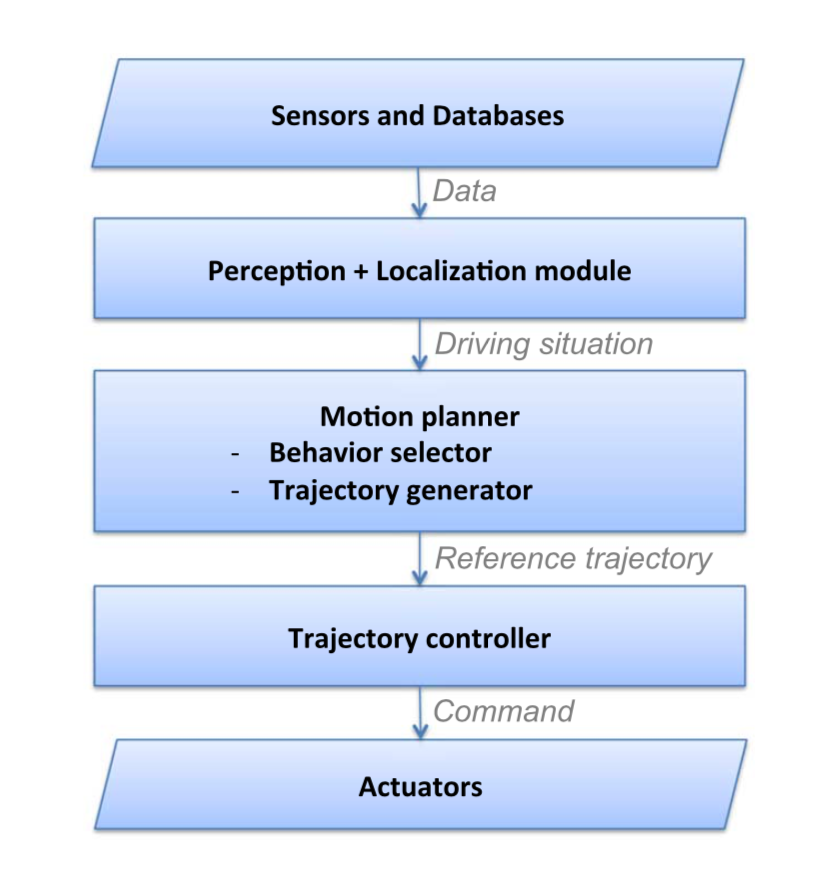
\includegraphics[width=0.5\textwidth]{figs/ch3/standard-architecture}
\caption{Standard Architecture of Autonomous Vehicle.}
\label{fig:std-archi}
\end{figure}

\begin{itemize}
\item The "Perception + Localization" module combines data received from sensors and digital maps to estimate some relevant features representing the driving situation (e.g. position of other vehicles, road geometry).
\item The "Motion planner" selects the appropriate high-level behavior (e.g. car following, lane changing) and generates a trajectory corresponding to that behavior.
\item The "Trajectory controller" computes the steering and acceleration commands with the objective to follow the reference trajectory as closely as possible. These commands are sent to the actuators.
\end{itemize}

This architecture has been successfully used in the field of terrestrial robotics for decades. Our autonomous driving framework inherits the most of it and replaces the motion planner with a trained driver model, which will be described in detail in Chapter 4.

The driver model can be designed independently and can be modified at any time without impacting the performance of the other. This feature is particularly useful if one wants to adjust the car's driving style over time: the driver model can learn continuously, or be replaced, without having to readjust any other module. One could also imagine extending the architecture in Fig. \ref{fig:proposed-architecture} to take advantage of cloud-based computing and learn new models based on data collected from millions of drivers.

\begin{figure}[h]
\centering
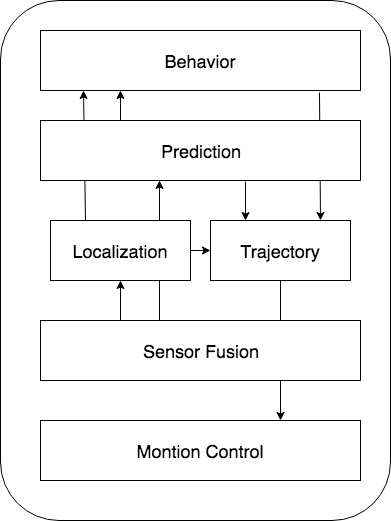
\includegraphics[width=0.5\textwidth]{figs/ch3/architecture}
\caption{Standard Architecture of Autonomous Vehicle Control.}
\label{fig:proposed-architecture}
\end{figure}

The framework proposed above is general and can be applied to a variety of driving scenarios. We will implement and test it for the longitudinal and lateral control of an autonomous vehicle during lane keeping and lane changing. In this scenario, the commanded input is the acceleration and steering of the vehicle. The system is aiming for constructing at least the following modules or functions.

% Topics
\begin{itemize}
\item \textbf{Path following} Detecting and determining a path/lane to follow, and following it.
\item \textbf{Lane and obstacle detection} Detecting driving lanes and obstacles to successfully navigate them.
\item \textbf{ACC} Detect a leading vehicle or a  trailing vehicle and maintain a safe distance and speed.
\item \textbf{Adaptive braking} Braking system adapts braking to different driving conditions to improve response time, overall safety, etc.
\end{itemize}

%%%%%%%%%%%%%%%%%%%%%%%%%%%%%%%%%%%%%%%%%%%
\section{Motion Planner}

%%%%%%%%%%%%%%%%%%%%%%%%%%%%%%%%%%%%%%%%%%%
\subsection{Longitudinal Control Problem}

We define the following variables to represent the relative motion of the autonomous vehicle (referred to as the "ego vehicle") and the vehicle located ahead or behind in the same lane as the autonomous vehicle (referred to as the "preceding vehicle" or the "trailing car").

\begin{itemize}
\item $\epsilon = [d_t, v_t]$ is the state of the ego vehicle at time \textit{t}, where $d_t \in R^+$ is the longitudinal position of the ego vehicle in a road-aligned coordinate system, and $v_t \in R^+$ is the longitudinal velocity of the ego vehicle.
\item $\epsilon = [d_t^p, v_t^p]$ is the state of the preceding vehicle at time \textit{t}, where $d_t \in R^+$ is the longitudinal position of the preceding vehicle in a road-aligned coordinate system, and $v_t \in R^+$ is the longitudinal velocity of the preceding vehicle.
\item $\epsilon = [d_t^t, v_t^t]$ is the state of the trailing vehicle at time \textit{t}, where $d_t \in R^+$ is the longitudinal position of the trailing vehicle in a road-aligned coordinate system, and $v_t \in R^+$ is the longitudinal velocity of the trailing vehicle.
\item $z_t =  [d_t^{pr}, d_t^{tr}, v_t^p, v_t^t, v_t^t]$ are the features representing the current driving situation at time \textit{t} , to be used by the driver model to generate an appropriate acceleration command. $d_t^{pr} = d_t^p - d_t$ is the relative distance to the preceding vehicle and $d_t^{tr} = d_t^t - d_t$ is the relative distance to the preceding vehicle.
\end{itemize}

At each time step \textit{t} , the driver model generates an acceleration command. This acceleration command is used by the trajectory generator to compute a target velocity as a reference. The controller solves a constrained optimization problem over the prediction horizon , and generates a planned velocity sequence which guarantees the safety of the vehicle.

%%%%%%%%%%%%%%%%%%%%%%%%%%%%%%%%%%%%%%%%%%%
\subsection{Lateral Control Problem}

We define a one-dimensional array with boolean values to represent the lateral position of the autonomous vehicle in a 3-lane highway scenario.

\begin{itemize}
\item $lane = [false, true, false]$ , for example, represents the vehicle locates at the middle lane at time \textit{t}.
\end{itemize}

\begin{figure}[h]
\centering
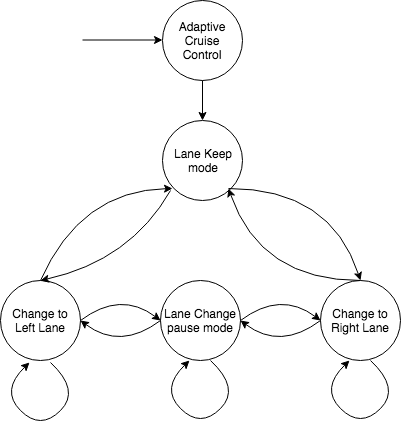
\includegraphics[width=0.7\textwidth]{figs/ch3/state-machine}
\caption{The finite state machine for lateral motion control.}
\label{fig:fsm}
\end{figure}

At each time step \textit{t} , the driver model, with the information above together with the other vehicle in its left and right lanes, generates a change lane or a keep lane command. The proposed algorithm will encourage the ego vehicle to change to a different lane neighboring to it when the target lane has better driving condition and to keep the current lane if else. To avoid conflict two lane changing commands which are too close, the lateral control would stay the current state for a period of time for the lane change to finish. Within the time period, new lane change or lane keep commands would be ignored. By this idea, it becomes a rule-based controller, sometimes referred to as "?nite state machine (FSM)", as shown in Fig. \ref{fig:fsm}. FSM has its own advantages, including:

\begin{enumerate}
\item \textbf {Clear in structure:} the controller is based on "if-then-else" logic, which is explicitly readable, so that the controller's behavior can be relatively easily predicted; 
\item \textbf {Easy to calibrate:} a FSM usually has a ?nite number of parameters, so that it is easy to calibrate and optimize;
\item \textbf {More reliable:} A well-calibrated FSM is usually more reliable, compared to some other frameworks, e.g., based on function approximation techniques as used in machine learning-based approaches.  
\end{enumerate}

%%%%%%%%%%%%%%%%%%%%%%%%%%%%%%%%%%%%%%%%%%%
\section{Trajectory Generator}

\subsection{Trajectory Planning}

The proposed Trajectory Generator is used to generate a safe and comfortable path (with an appropriate speed and acceleration) from an initial position towards a destination, while complying with a global route and map. Our method aims to resolve local path planning problems based on a global route and map. The global route is obtained by the high precision navigation system, and the map is downloaded from the Internet. The map is composed of a set of waypoints on the road edges and topology that describes the relationships between connected roads, as shown in Fig. \ref{fig:center-line}. The process by which the map is obtained falls outside the scope of this thesis. Therefore, the maps used in this paper are predefined in our simulations.

\begin{figure}[h]
\centering
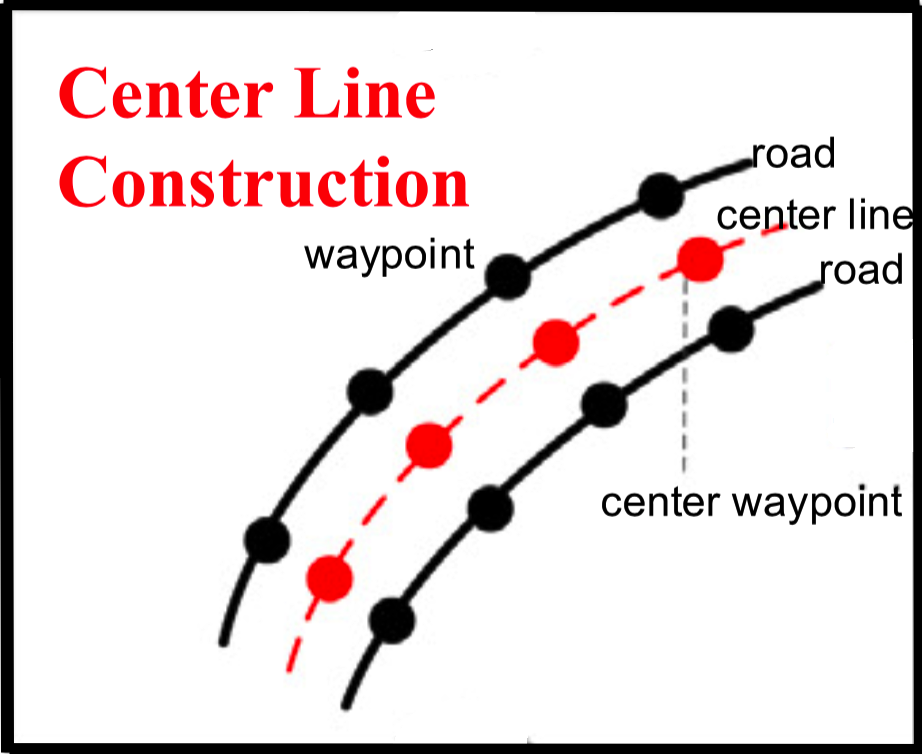
\includegraphics[width=0.5\textwidth]{figs/ch3/center-line}
\caption{The global route and the waypoints.}
\label{fig:center-line}
\end{figure}

The dynamic path planning process includes three stages: center line construction, path candidate generation, and path selection. These are performed on the basis of perceived information. The center line of the road is constructed from the center waypoints, which are several waypoints captured from the map and aligned to the center line of the lane, using the method of cubic spline fitting. The path candidates, which are also described by the cubic spline, are generated by adjusting the lateral offset to the center line using the information for the current vehicle position, speed, and direction in a road-aligned coordinate system. During path selection, the costs of static safety, comfortability, and dynamic safety are taken into account, and are combined with information on road edges, and static and moving obstacles for selecting the optimal path. Our method provides not only the selected path, but also the appropriate speed for the vehicle maneuvering system. In this project, the proposed dynamic path planning algorithm is executed 50 times per second, and a new path is generated from the current vehicle position at every time step. 

\subsection{A road-aligned coordinate system: Frenet Coordinate}

As we have mentioned several times in the previous section, a road-aligned coordinate system is needed to have a better view on the global and local trajectories. A well known one is the Frenet coordinate, which asserts invariant tracking performance under the action of the special Euclidean group $SE(2) := SO(2) \times \mathbb{R}^2$. Here, we will apply this coordinate system in order to be able to combine different lateral and longitudinal cost functionals for different tasks as well as to mimic human-like driving behavior on the highway. As depicted in Fig. \ref{fig:traj-generation}, the moving reference frame is given by the tangential and normal vector $\overrightarrow{t_r}$, $\overrightarrow{n_r}$ at a certain point of some curve referred to as the center line in the following. This center line represents either the ideal path along the free road, in the most simple case the road center, or the result of a path planning algorithm for unstructured environments \cite{Frenet2008}. Rather than formulating the trajectory generation problem directly in Cartesian Coordinates $\overrightarrow{x}$, we switch to the proposed dynamic reference frame and seek to generate a one-dimensional trajectory for both the root point $\overrightarrow{r}$ along the center line and the perpendicular offset \textit{d} with the relation

\begin{figure}[h]
\centering
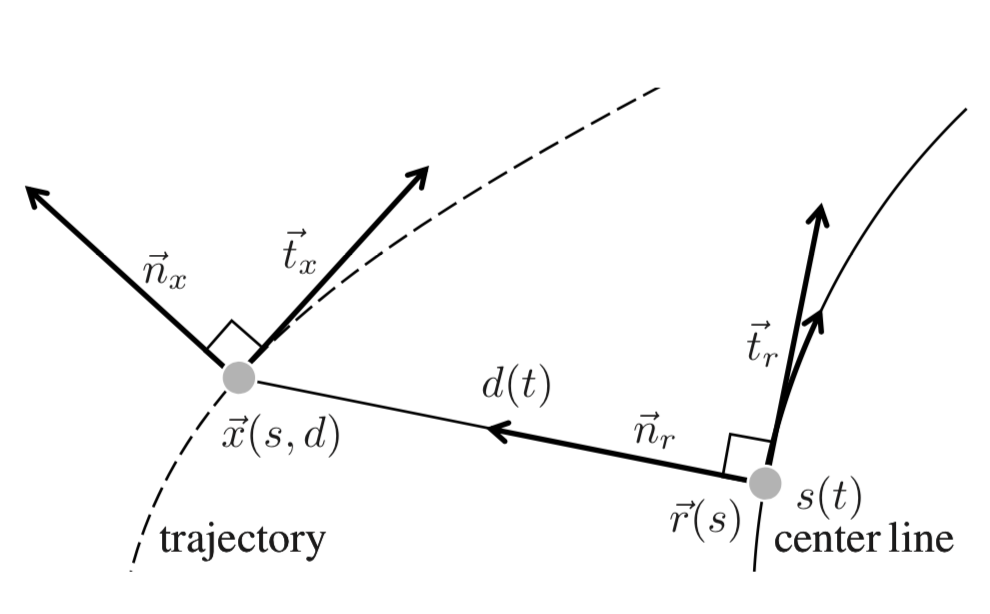
\includegraphics[width=0.5\textwidth]{figs/ch3/traj-generation}
\caption{Trajectory generation in Frenet coordinate.}
\label{fig:traj-generation}
\end{figure}

\subsubsection{Frenet Coordinates}

Frenet Coordinates are a way of representing position on a road in a more intuitive way than traditional $(x,y)$ Cartesian Coordinates. With Frenet coordinates, we use the variables $s$ and $d$ to describe a vehicle's position on the road. The $s$ coordinate represents distance along the road (also known as longitudinal displacement) and the $d$ coordinate represents side-to-side position on the road (also known as lateral displacement). Imagine a curvy road like in Fig. \ref{fig:curve-in-cartesian} with a Cartesian coordinate system laid on top of it.

\begin{figure}[h]
\centering
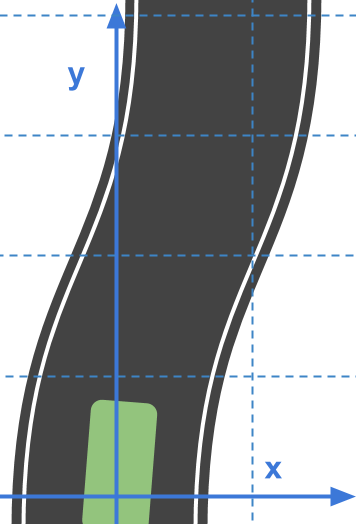
\includegraphics[width=0.25\textwidth]{figs/ch3/curve-in-cartesian}
\caption{A curve road in Cartesian coordinate.}
\label{fig:curve-in-cartesian}
\end{figure}

Using these Cartesian coordinates, we can try to describe the path a vehicle would normally follow on the road as shown in Fig. \ref{fig:curve-in-cartesian-wp}.

\begin{figure}[h]
  \centering
    \begin{minipage}{.5\textwidth}
        \centering
        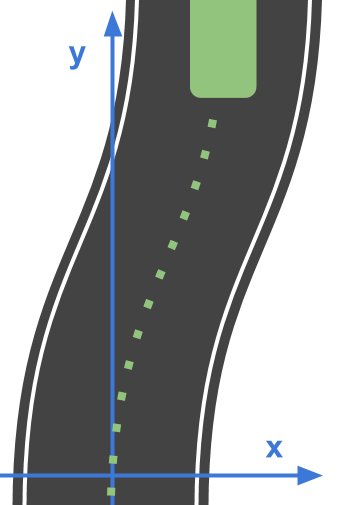
\includegraphics[height=2.4in]{figs/ch3/curve-in-cartesian-with-waypoints}
    \end{minipage}
    ~
    \begin{minipage}{.5\textwidth}
       \centering
      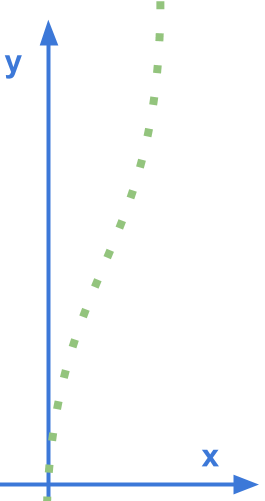
\includegraphics[height=2.4in]{figs/ch3/waypoints-in-cartesian}
     \end{minipage}
\caption{A curve road in Cartesian coordinate with waypoints.}
\label{fig:curve-in-cartesian-wp}
\end{figure}

And notice how curvy that path is. If we wanted equations to describe this motion it wouldn't be easy. Ideally, it should be mathematically easy to describe such common driving behavior. Now instead of laying down a normal Cartesian grid, we would refer to Frenet coordinate system as below in Fig. \ref{fig:curve-in-frenet}.

\begin{figure}[h]
\centering
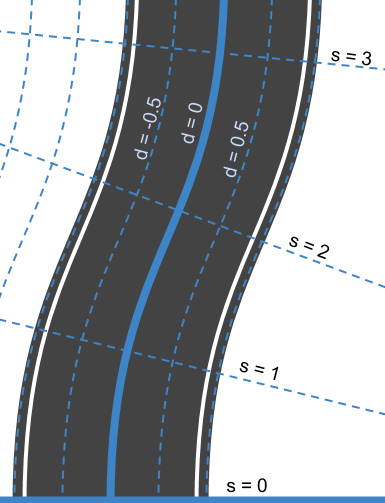
\includegraphics[width=0.25\textwidth]{figs/ch3/curve-in-frenet}
\caption{Curve in Frenet coordinate system.}
\label{fig:curve-in-frenet}
\end{figure}

Here, we've defined a new system of coordinates. At the bottom we have s=0 to represent the beginning of the segment of road we are thinking about and $d=0$ to represent the center line of that road. To the left of the center line we have negative $d$ and to the right $d$ is positive. Then a typical trajectory would look like in Fig. \ref{fig:curve-in-frenet-wp} when presented in Frenet coordinate.

\begin{figure}[h]
  \centering
    \begin{minipage}{.5\textwidth}
        \centering
        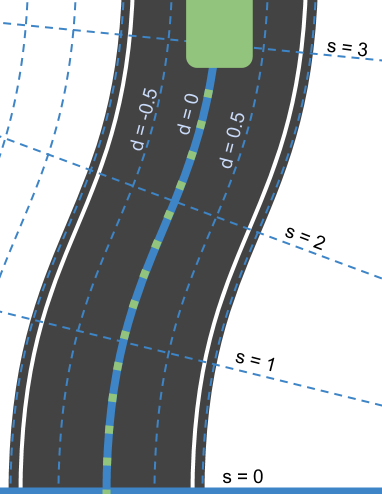
\includegraphics[height=2.4in]{figs/ch3/curve-in-frenet-with-waypoints}
    \end{minipage}
    ~
    \begin{minipage}{.5\textwidth}
       \centering
      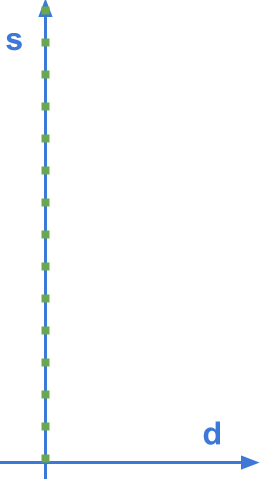
\includegraphics[height=2.4in]{figs/ch3/waypoints-in-frenet}
     \end{minipage}
\caption{A curve road in Frenet coordinate with waypoints.}
\label{fig:curve-in-frenet-wp}
\end{figure}

It looks straight! In fact, if this vehicle were moving at a constant speed of $v_0$ we could write a mathematical description of the vehicle's position as:

\begin{subequations} \label{eq:math-in-frenet}
\begin{align}
s(t) &= v_0^t \\
d(t) &= 0
\end{align}
\end{subequations}

\begin{figure}[h]
\centering
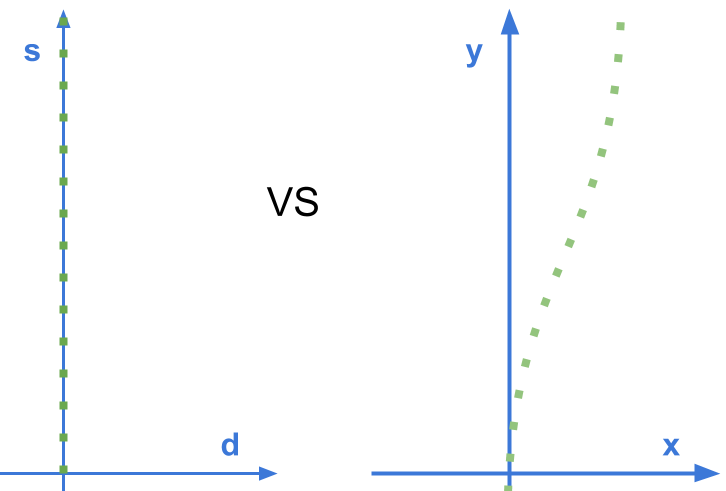
\includegraphics[height=2.8in]{figs/ch3/frenet-final}
\caption{Comparison display in Frenet and Cartesian coordinate systems.}
\label{fig:frenet-final}
\end{figure}

Straight lines are so much easier than curved ones.

\subsection{Reference path generation}

The path is the trajectory guiding the vehicle to follow a global route and avoid obstacles. The arc length $s$ indicates the traveling distance on the global route, and the offset $\rho$ can be used to measure the distance between the vehicle and the road edge.

To use the direction and curvature of the center line, it is necessary to find the position of the vehicle on the reference waypoints. We first map the vehicle position from the Cartesian coordinate system to the Frenet coordinate system, and then determine the closest point of the center line $p_0$, which has the minimum distance $\rho_{min}$. In this paper, a method combining quadratic minimization and Newton's method is used to find $p_0$.

\begin{figure}[h]
\centering
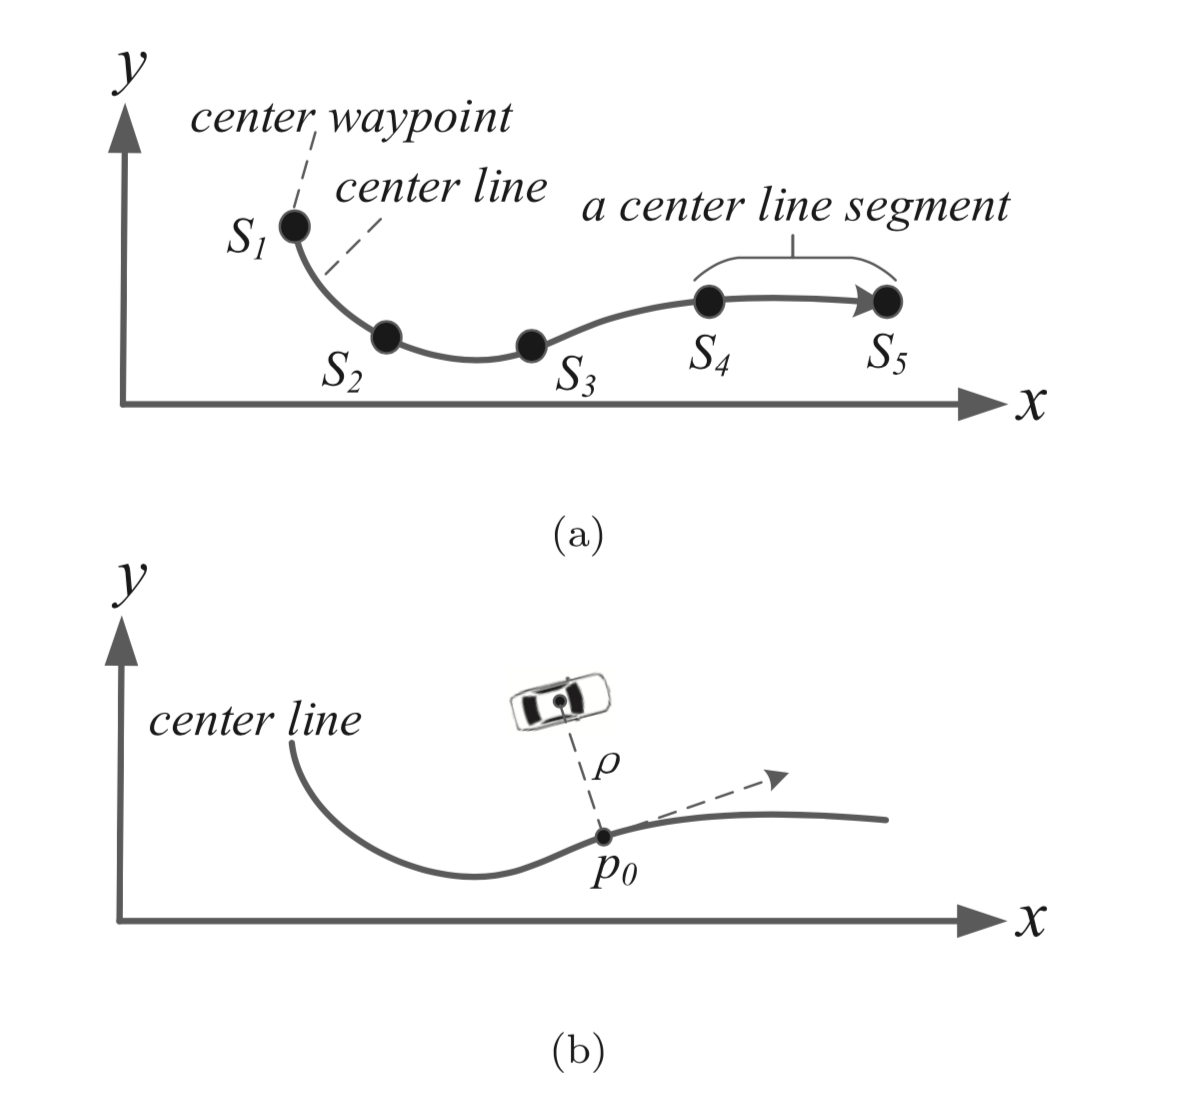
\includegraphics[height=2.8in]{figs/ch3/location-on-center-line}
\caption{Vehicle localization on the center line. (a) Center waypoints and center line segments, (b) localization on the center line.}
\label{fig:loc-line}
\end{figure}

To generate path candidates, the curvature of each path is determined by the lateral offset $d$ of the path, based on the curvature of the center line. As shown in Fig. \ref{fig:loc-line} (a), $p_{init}$ is the original point on the center line. $p_{start}$ and $p_{end}$ are the start and end points on the center line, respectively, for one step of planning. $p_{veh}$ is the start point of the vehicle. $p_1$ to $p_5$ are the end points of five path candidates, and are indicated by $r_1$ to $r_5$. It is obvious that only $r_2$; $r_4$, and $r_5$ are available and free of obstacles. The reason for this availability lies with the differences between the offset from the path candidate to the center line and the offset from the obstacle to the center line. Meanwhile, the positions of the obstacle and the vehicle on the center line can be expressed by the arc length $s$.

Path candidates are generated in the Frenet coordinate system, but path planning results must be mapped into a Cartesian coordinate system to convey to the maneuvering system. Path candidate points in the Cartesian coordinate system can be represented with respect to the arc length of the center line as Eq. (6) [43].

%%%%%%%%%%%%%%%%%%%%%%%%%%%%%%%%%%%%%%%%%%%
\section{Path Flowing}

\subsection{Waypoint Follower Node}
The waypoint follower node uses the $/final_waypoints$ data to publish $/twist_cmd$ for the dbw node to use. The node implementation uses an open source implementation of pure pursuit algorithm from Autoware. (https://github.com/CPFL/Autoware)

%%%%%%%%%%%%%%%%%%%%%%%%%%%%%%%%%%%%%%%%%%%
\section{Drive By Wire}

\subsection{Drive By Wire (DBW) Node}

An autonomous car require that actuators that control the motion of the vehicle, can be interacted with electronically. Therefore a drive-by-wire system is needed. A drive-by-wire system replaces the mechanical systems in a traditional vehicle by using electrical/electronic (E/E) systems to perform fundamental vehicle functions.

The drive-by-wire system includes steer-by-wire, brake-by-wire and throttle-by-wire. The "by-wire" expression means that the information, from the sensor to the actuator of the different systems, is transferred electronically through wires and not by traditional hydraulic systems or mechanically through struts or shafts.

The advantage of using drive-by-wire rather than mechanical systems is that reduction of cost, moving parts and weight can be achieved. Since the steering rack can be removed, the car?s shock impact, in case of a collision, can be improved. Using an electrical based system will also increase the information flow and ease up the interconnect between different components in the car, facilitating the use of safety functions such as; ABS (anti-lock brake system), ESP (electronic stability programme), etc.


The purpose of the drive by wire node is to publish commands to the vehicle actuators: steering wheel, accelerator, and break. The node subscribes to the following nodes:

${/current_velocity}$

$/twist_cmd$

$/vehicle/dbw_enabled$

It uses information from $current_velocity$ and $twist_cmd$ to determine the values to be sent to the actuators, while $/vehicle/dbw_enabled$ topic is only used to determine if drive-by-wire is being overridden, in which point it will stop publishing any message, and ignore the received messages.

The node delegates the actuator's value to the $twist_controller$ class, which returns a value for each of the actuators.

\subsubsection{Twist Controller}
The twist controller is initialized with values based on the vehicle configuration, as steer ratio and vehicle mass, and implements a single method control, which receives the vehicle target position and current velocity, and will return a value for acceleration, braking, and steering. It will in turn, delegate the calculation for each of those values to the $throttle_controller$, $brake_controller$, and $yaw_controller$. The $yaw_controller$ calculates a steering angle for every update, while the twist controller will calculate the position error (current - target) to determine if braking or acceleration should be engaged. If the error is positive, the throttle controller is used, while a negative error will be sent to the brake PID.

1) Throttle Controller ($throttle_controller.py$)
The throttle is initialized with a min and max acceleration values. It uses a PID controller to determine the amount of acceleration or decelaration to be given based on the difference between the target velocity and the current velocity.

2) Braking Controller ($braking_controller.py$)
The brake controller calculates the amount of torque to be sent to the brake by multiplying the vehicle mass, wheel radius and aceleration.

3) Steering Controller ($yaw_controller.py$)
The steering controller calculates the amount of steering it should send to the actuator using the target linear and angular velocity, taking into account the steer ratio of the vehicle.





%\bibliographystyle{plainnat}
%\markright{\textit{Bibliography}}
%\renewcommand{\chaptername}{}
%\bibliography{KL-Thesis}

%\end{flushleft}
%\vfill
